\documentclass{article}

% if you need to pass options to natbib, use, e.g.:
%     \PassOptionsToPackage{numbers, compress}{natbib}
% before loading neurips_2021

% ready for submission
% \usepackage{neurips_2021}

% to compile a preprint version, e.g., for submission to arXiv, add add the
% [preprint] option:
% NB add nonatbib to avoid bibtex compatibility error
\usepackage[preprint,nonatbib]{neurips_2021} 

% to compile a camera-ready version, add the [final] option, e.g.:
%     \usepackage[final]{neurips_2021}

% to avoid loading the natbib package, add option nonatbib:
%    \usepackage[nonatbib]{neurips_2021}

\usepackage[utf8]{inputenc} % allow utf-8 input
\usepackage[T1]{fontenc}    % use 8-bit T1 fonts
\usepackage[hidelinks]{hyperref}       % hyperlinks
\usepackage{url}            % simple URL typesetting
\usepackage{booktabs}       % professional-quality tables
\usepackage{amsfonts}       % blackboard math symbols
\usepackage{nicefrac}       % compact symbols for 1/2, etc.
\usepackage{microtype}      % microtypography
\usepackage{xcolor}         % colors
\usepackage{lipsum}         % filler

\usepackage{amsmath,amssymb,amsthm}
\usepackage{graphicx}

\usepackage[natbib,hyperref,sorting=none]{biblatex}
% \usepackage[backend=bibtex,doi=true,style=numeric,maxnames=3,maxbibnames=6]{biblatex}
%  \usepackage[backend=bibtex,style=numeric,natbib=true]{biblatex} 
%% REFERENCES
\addbibresource{sections/06-References.tex} 

\title{Evaluation of self-driving cars using \\ CNNs in the rain}

% The \author macro works with any number of authors. There are two commands
% used to separate the names and addresses of multiple authors: \And and \AND.
%
% Using \And between authors leaves it to LaTeX to determine where to break the
% lines. Using \AND forces a line break at that point. So, if LaTeX puts 3 of 4
% authors names on the first line, and the last on the second line, try using
% \AND instead of \And before the third author name.

\author{
    Daniel Sikar \\
    School of Mathematics, Computer Science \\ and Engineering \\
    City, University of London \\
    \texttt{daniel.matvienko-sikar@city.ac.uk} \\
    \And
    Artur d’Avila Garcez  \\
    School of Mathematics, Computer Science \\ and Engineering \\
    City, University of London\\
    \texttt{a.garcez@city.ac.uk} \\
}

\begin{document}

\maketitle

%% ABSTRACT

\begin{abstract}

%The abstract paragraph should be indented \nicefrac{1}{2}~inch (3~picas) on
%  both the left- and right-hand margins. Use 10~point type, with a vertical
%  spacing (leading) of 11~points.  The word \textbf{Abstract} must be centered,
%  bold, and in point size 12. Two line spaces precede the abstract. The abstract

%  must be limited to one paragraph.
  



%%% APPLICATION AND SUCCESS STORY OF CONVNETS 
%%% ConvNets has found success in diverse areas.
%%% Deep learning has found successful application in diverse areas
%%% including end-to-end self-driving cars, where a trained model is given an image and outputs values such as steering and throttle.

%%% THE PROBLEM WE ARE DEALING WITH - CONVNETS LACKING ROBUSTNESS E.G. ONE-PIXEL-ATTACKS, RANDOM LABELS (BENGIO ET AL)
% However, there is a problem - noisy images

%%% WHAT WE DID - maybe leave the nitty gritty for later e.g. Unity 3D ?
This project investigates the effect of rainy images on the performance of end to end convolutional neural networks (CNNs) applied to self-driving cars, using public domain real-world datasets, as well as data synthetically generated by the Unity 3D gaming engine. 
%%% WHAT WE FOUND

% we need an angle here on the bigger picture of end-to-end learning of which self-driving cars training with behavioural learning are a specific case.
% Like a survey on end-to-end applications

% TODO end-to-end applications, one or two paragraphs, maybe in the intro or context.


%%% Results suggest that random noise does have a detrimental effect on network performance which may be mitigated by 

CNNs have become state-of-the-art in supervised image classification tasks, and are used for regression tasks in both \textit{pipelined} and \textit{end-to-end} neural network architectures. the former relying on a fusion of image and sensor data the latter on images alone, to determine steering and movement output.  
However, CNNs applied to image classification have been shown to lack robustness when, given noisy images, in some cases a single pixel change, are known to output incorrect results that for humans would have been obviously the same as the denoised versions.
As deep learning models, be it CNNs, Recurrent Neural Networks or Deep Reinforcement Learning Networks rely increasingly on computer vision for robotics in general, and for self-driving cars in particular, it is important to evaluate the effect of noisy data, such as images containing rain, used by such models.
This study, as far as current literature searches show, is the first of its kind, and provides a novel testing environment that is able to subject self-driving CNN architectures to different rain levels, which may inform design decisions relating to safety in self-driving, as well as robotics relying on computer vision, as well as any Machine Learning/Artificial intelligence application relying on game engines for training and testing data, where the trained model is to be deployed in environments subject to image noise.
% WHAT WE FOUND
% Results suggest that image pre-processing may be used to neutralise the effect of noise such as rainy images.

% This study is to the best of my knowledge the first of its kind.

%%% By training and testing resulting models with the Unity 3D game engine, we provide

\end{abstract}

%% INTRODUCTION
\section{Introduction}

We are tackling a hard problem here.

%% METHODS
\section{Methods}




\begin{figure}[htbp]
  \centering
  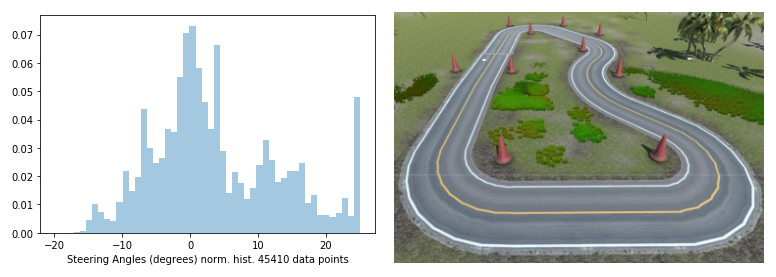
\includegraphics[width=\textwidth]{Figures/GeneratedTrackPlusHistogram.png}
 \caption{
 Normalized histogram of Unity 3D SDSandbox steering angles for 45410 image frames. The corresponding track (small\_looping\_couse) is shown on the right
 }
 \label{fig:GeneratedTrackPlusHist}
\end{figure}

\begin{figure}[htbp]
 \centering 
 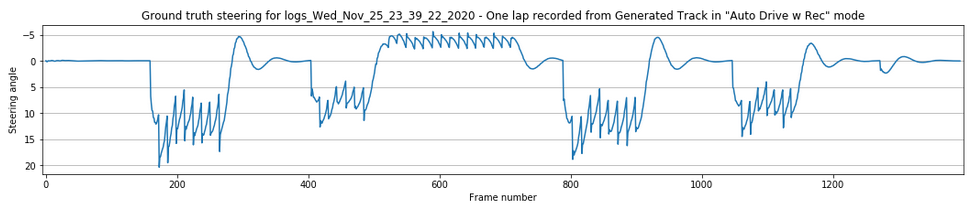
\includegraphics[width=\textwidth]{Figures/genTrackOneLap_logs_Wed_Nov_25_23_39_22_2020_ground_truth_steering_angles.png}
 \caption{Ground truth steering values for logs\_ Wed\_ Nov\_ 25\_ 23\_ 39\_ 22\_ 2020 recorded log.}
 \label{fig:genTrackOneLap_logs_Wed_Nov_25_23_39_22_2020_ground_truth_steering_angles} 
\end{figure}

\begin{figure}[htbp]
\centering
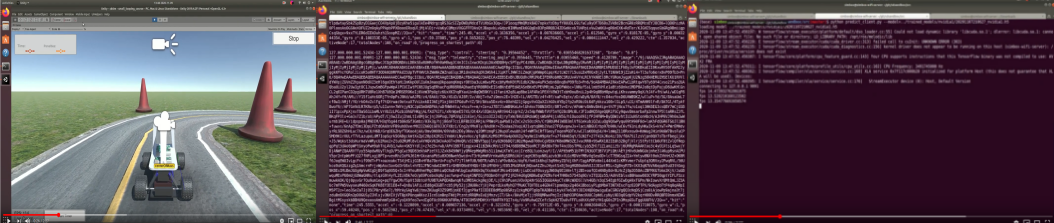
\includegraphics[width=\textwidth]{Figures/SimTCPPred.png}
\caption{Stills of video \url{https://youtu.be/9z0mMtOnUUc} showing left to right: SDSandbox simulated car going around the Generated Track course, TCP Debug (tcpflow) and prediction engine (predict\_ client.py) running}
\label{fig:SimTCPPred}
\end{figure}

\begin{figure}[htbp]
 \centering 
 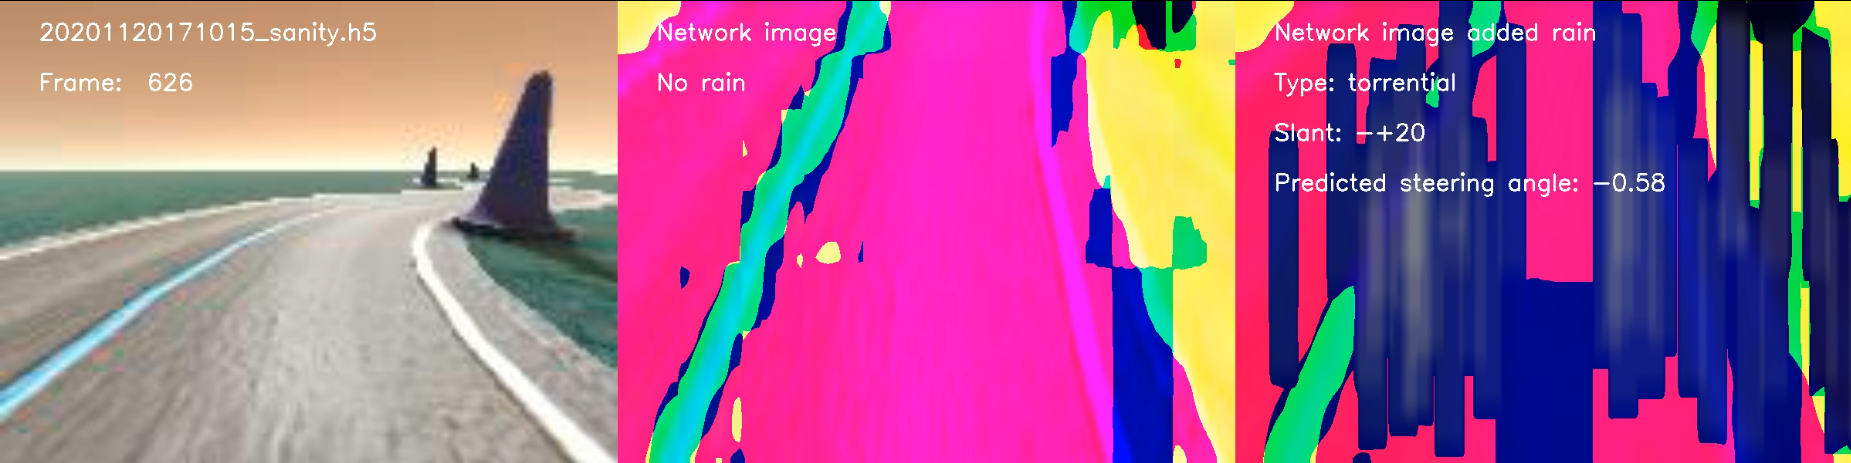
\includegraphics[width=\textwidth]{Figures/tcpflow_Run43.png}
 \caption{Video still showing left to right, the acquired image supplied by the simulator, a processed network image with no rain and the same image with torrential rain added. This last being the image presented to the network. A video was recorded in run \ref{app_res:43}, \url{https://youtu.be/57jwwcjbfdE}, showing the model driving off the track.}
 \label{fig:tcpflow_Run43} 
\end{figure}

%%%%%%%%%%%%%%%%%%%%%%%%%%%%%%%%%%%%%%%%%%%%%%%%%%
% Generated Road, sim on left and detail on right
%%%%%%%%%%%%%%%%%%%%%%%%%%%%%%%%%%%%%%%%%%%%%%%%%%

\begin{figure}[htbp]
 \centering 
 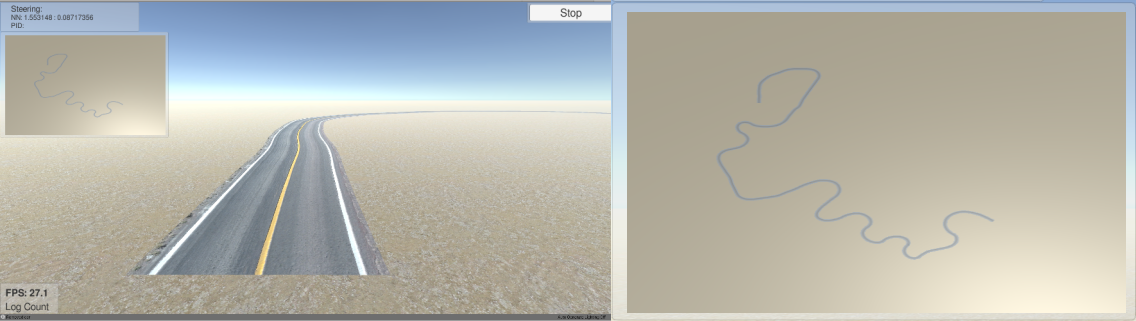
\includegraphics[width=\textwidth]{Figures/run-93-94-generated-road.png}
 \caption{The randomly generated Generated Road circuit used in runs 93 and 94. Left image is a view of the simulator as presented on computer desktop, the right image is the augmented detail showing the Generated Road circuit, the same inset on left image.}
 \label{fig:run-93-94-generated-road-res} 
\end{figure}

We created a simulation and got the network to predict the outcome.

The evaluation can be performed qualitatively using a simulator as described in (TODO MISSING REF) to observe the simulated vehicle self-driving with respect to oversteering and understeering, crashes providing pass/fail metric.

The proposed quantitive evaluation metric is \textit{goodness-of-steer}. In equation     \ref{eq:goodness_of_steer}:

\begin{equation}
    \label{eq:goodness_of_steer}
    g_s(p,g) = \frac{\sum_i^N \lvert p(i)-g(i) \rvert }{N} \times n_c
\end{equation}
where $p,g$ are prediction and ground truth arrays,  $N$ is the number of predictions and $n_c$ is the normalization constant (25 in example shown, 1 for values not normalized), which in this case is the maximum steering angle for the SDSandbox simulated vehicle. In plain english, $g_s$ is defined as the sum of the absolute value of the difference between prediction and ground truth values, divided by the number of predictions multiplied by a normalization constant, that is the steering error average over all predictions. 

%% EVALUATION
\section{Results}

%%%%%%%%%%%%%%%%%%
% RESULTS TABLE
%%%%%%%%%%%%%%%%%%

% Table generated with steerlib.py
\begin{table}[]
\begin{center}
\begin{tabular}{l l l l l l}
\hline
\multicolumn{6}{ c }{Goodness-of-steer results - Generated Track and Generated Road SDSandbox logs} \\ \hline

% 1 Log: Unity log location (image plus .json files)
% 1 Filename:   Download  D1  Udacity real world dataset
% 2 Model:    D2  Udacity simulator data
% 3 Rain Type: D3  Udacity real and simulator data
% 4 Slant: Turk dry/rainy Ford dataset
% 5.GOS: Goodness of steer

% Generated Track log number of image files
% $ ls -l ../../dataset/unity/genTrack/genTrackOneLap/logs_Wed_Nov_25_23_39_22_2020/*.jpg | wc -l
% 1394
% Generated Road log number of image files
% $ ls -l ../../dataset/unity/genRoad/logs_Fri_Jul_10_09_16_18_2020/*.jpg | wc -l
% 19679

\multicolumn{6}{c}{Generated Track log: logs\_ Wed\_ Nov\_ 25\_ 23\_ 39\_ 22\_ 2020 (1394 images)} \\ \hline
ID & Keras model file name & Model & Rain Type & Slant & $g_s$ \\ \hline
% GENERATED TRACK
1 & 20201207192948\_ nvidia2.h5 & nvidia2 :) &  & 0 & 1.68 * \\ \hline
2 & 20201207192948\_ nvidia2.h5 & nvidia2 & light & 0 & 2.12 \\ \hline
3 & 20201207192948\_ nvidia2.h5 & nvidia2 & heavy & 10 & 2.17 \\ \hline
4 & 20201207192948\_ nvidia2.h5 & nvidia2 & torrential & 20 & 2.30 \\ \hline
5 & 20201207091932\_ nvidia1.h5 & nvidia1 &  & 0 & 1.82 * \\ \hline
6 & 20201207091932\_ nvidia1.h5 & nvidia1 & light & 0 & 2.11 \\ \hline
7 & 20201207091932\_ nvidia1.h5 & nvidia1 & heavy & 10 & 2.13 \\ \hline
8 & 20201207091932\_ nvidia1.h5 & nvidia1 & torrential & 20 & 2.28 \\ \hline
9 & 20201207201157\_ nvidia\_ baseline.h5 & nvidia2\_ baseline &  & 0 & 2.32 * \\ \hline
10 & 20201207201157\_ nvidia\_ baseline.h5 & nvidia2\_ baseline & light & 0 & 3.12 \\ \hline
11 & 20201207201157\_ nvidia\_ baseline.h5 & nvidia2\_ baseline & heavy & 10 & 3.17 \\ \hline
12 & 20201207201157\_ nvidia\_ baseline.h5 & nvidia2\_ baseline & torrential & 20 & 3.39 \\ \hline
13 & 20201120171015\_ sanity.h5 & nvidia1 :( &  & 0 & 5.03 * \\ \hline
14 & 20201120171015\_ sanity.h5 & nvidia1 & light & 0 & 3.11 \\ \hline
15 & 20201120171015\_ sanity.h5 & nvidia1 & heavy & 10 & 3.07 \\ \hline
16 & 20201120171015\_ sanity.h5 & nvidia1 & torrential & 20 & 3.00 \\ \hline
% GENERATED ROAD
\multicolumn{6}{c}{Generated Road log:  logs\_ Fri\_ Jul\_ 10\_ 09\_ 16\_ 18\_ 2020 (19679 images)} \\ \hline
ID & Keras model file name & Model & Rain Type & Slant & $g_s$ \\ \hline
% NVIDIA2
17 & 20201207192948\_ nvidia2.h5 & nvidia2 :) &  & 0 & 2.99 * \\ \hline  % drove 16 minutes on this road 1 & https://youtu.be/z9nILq9dQfI
18 & 20201207192948\_ nvidia2.h5 & nvidia2 & light & 0 & 3.20 \\ \hline
19 & 20201207192948\_ nvidia2.h5 & nvidia2 & heavy & 10 & 3.22 \\ \hline
20 & 20201207192948\_ nvidia2.h5 & nvidia2 & torrential & 20 & 3.27 \\ \hline
% NVIDIA1
21 & 20201207091932\_ nvidia1.h5 & nvidia1 &  & 0 & 3.87 * \\ \hline
22 & 20201207091932\_ nvidia1.h5 & nvidia1 & light & 0 & 3.75 \\ \hline
23 & 20201207091932\_ nvidia1.h5 & nvidia1 & heavy & 10 & 3.70 \\ \hline
24 & 20201207091932\_ nvidia1.h5 & nvidia1 & torrential & 20 & 3.57 \\ \hline
% NVIDIA_BASELINE
25 & 20201207201157\_ nvidia\_ baseline.h5 & nvidia2\_ baseline :( &  & 0 & 5.51 * \\ \hline
26 & 20201207201157\_ nvidia\_ baseline.h5 & nvidia2\_ baseline & light & 0 & 4.97 \\ \hline
27 & 20201207201157\_ nvidia\_ baseline.h5 & nvidia2\_ baseline & heavy & 10 & 4.98 \\ \hline
28 & 20201207201157\_ nvidia\_ baseline.h5 & nvidia2\_ baseline & torrential & 20 & 5.05 \\ \hline
% SANITY (NVIDIA1)
29 & 20201120171015\_ sanity.h5 & nvidia1 &  & 0 & 3.85 * \\ \hline
30 & 20201120171015\_ sanity.h5 & nvidia1 & light & 0 & 3.06 \\ \hline
31 & 20201120171015\_ sanity.h5 & nvidia1 & heavy & 10 & 3.05 \\ \hline
32 & 20201120171015\_ sanity.h5 & nvidia1 & torrential & 20 & 3.02 \\ \hline
%   compare to genTrackOneLap_logs_Wed_Nov_25_23_39_22_2020_ground_truth_steering_angles.png
\end{tabular}
\end{center}
\caption{Goodness-of-Steer $g_s$ results for best performing nvidia2 and nvidia1, plus "sanity" and nvidia\_ baseline for comparison, obtained from one lap of Generated Track (logs\_ Wed\_ Nov\_ 25\_ 23\_ 39\_ 22\_ 2020, rows 1 to 16) and one stretch of Generated Road (logs\_ Fri\_ Jul\_ 10\_ 09\_ 16\_ 18\_ 2020, rows 17 to 32). Asterisks in $g_s$ column indicate dry weather. Smiley face :) in Model column indicate best (lowest) $g_s$ score. Sad face :( in Model column indicates worst (highest) $g_s$ scores. The logs containing labelled image data used to compute the $g_s$ scores were generated with Unity intensity multiplier 1 and Skybox-Material set to Default-Skybox, the default sunny dry weather.}
\label{table:goodness-of-steer}
\end{table}

Table \ref{table:goodness-of-steer} shows Goodness-of-Steer results obtained for 32 sets of predictions, for four networks and two SDSandbox track logs, that is, the results were generated by running predictions on synthetic datasets, which contain ground truth steering values, like plotted in Figure \ref{fig:genTrackOneLap_logs_Wed_Nov_25_23_39_22_2020_ground_truth_steering_angles}. It is important to stress these are not realtime predictions, and the Unity simulator was not running in this case.

The networks are the best performing nvidia2 (obtained in run 62 - \ref{app_res:62}), the second best performing nvidia1 (obtained in run 49 - \ref{app_res:49}), "sanity check" (obtained in run 36 - \ref{app_res:36}) and nvidia\_ baseline (obtained in run 68 - \ref{app_res:68}). Table data and steering angle plots was generated with steerlib.py script written for this project. The track logs are for Generated Track (one lap) and Generated Road (one stretch). There are 32 rows, each sequence of four (1-4, 5-8 and so on) representing one model subject to sunny weather followed by 3 types of rain predicting steering angles for one log. 

nvidia2 predicted steering angle values used to generate $g_s$ scores in rows 1, 2, 3 and 4, for the Generated Track log are plotted in Figure  \ref{fig:sa_Generated_Track_20201207192948_nvidia2.h5}. The "no rain" predictions in row 1 (orange line on the plot), which has the lowest overall (1.68) $g_s$ score, is clearly the closest to the ground truth blue line, while the predictions for images containing light, heavy and torrential rain are tightly overlapped (green, red an violet lines, $g_s$ scores 2.12, 2.17, 2.30 respectively) are understeering on all turns (slightly above right turn ground truth plot in right turn sections and below ground truth plot in the left turn section. The understeering aspect was also noted in realtime predictions with respect to rainy predictions compared to best-run dry weather predictions as shown in Figures \ref{fig:sa_GeneratedTrackintensitymultiplier1_20201207192948_nvidia2}, 
\ref{fig:sa_GeneratedTrackintensitymultiplier4_20201207192948_nvidia2} and 
\ref{fig:sa_GeneratedTrackintensitymultiplier8_20201207192948_nvidia2}.

Note that publication-quality tables \emph{do not contain vertical rules.} We
strongly suggest the use of the \verb+booktabs+ package, which allows for
typesetting high-quality, professional tables:
\begin{center}
  \url{https://www.ctan.org/pkg/booktabs}
\end{center}
This package was used to typeset Table~\ref{sample-table}.

\begin{table}
  \caption{Generated Track Results}
  \label{generated-track-table}
  \centering
  \begin{tabular}{llllll}
    \toprule
    ID & Model file name & Model & Rain Type & Slant & $g_s$ \\ 
    \midrule
    % GENERATED TRACK
    1 & 20201207192948\_ nvidia2.h5 & nvidia2 :) &  & 0 & 1.68 * \\ 
    2 & 20201207192948\_ nvidia2.h5 & nvidia2 & light & 0 & 2.12 \\ 
    3 & 20201207192948\_ nvidia2.h5 & nvidia2 & heavy & 10 & 2.17 \\ 
    4 & 20201207192948\_ nvidia2.h5 & nvidia2 & torrential & 20 & 2.30 \\ 
    5 & 20201207091932\_ nvidia1.h5 & nvidia1 &  & 0 & 1.82 * \\ 
    6 & 20201207091932\_ nvidia1.h5 & nvidia1 & light & 0 & 2.11 \\ 
    7 & 20201207091932\_ nvidia1.h5 & nvidia1 & heavy & 10 & 2.13 \\ 
    8 & 20201207091932\_ nvidia1.h5 & nvidia1 & torrential & 20 & 2.28 \\ 
    9 & 20201207201157\_ nvidia\_ baseline.h5 & nvidia2\_ baseline &  & 0 & 2.32 * \\ 
    10 & 20201207201157\_ nvidia\_ baseline.h5 & nvidia2\_ baseline & light & 0 & 3.12 \\ 
    11 & 20201207201157\_ nvidia\_ baseline.h5 & nvidia2\_ baseline & heavy & 10 & 3.17 \\ 
    12 & 20201207201157\_ nvidia\_ baseline.h5 & nvidia2\_ baseline & torrential & 20 & 3.39 \\ 
    13 & 20201120171015\_ sanity.h5 & nvidia1 :( &  & 0 & 5.03 * \\ 
    14 & 20201120171015\_ sanity.h5 & nvidia1 & light & 0 & 3.11 \\ 
    15 & 20201120171015\_ sanity.h5 & nvidia1 & heavy & 10 & 3.07 \\ 
    16 & 20201120171015\_ sanity.h5 & nvidia1 & torrential & 20 & 3.00 \\ 
    \bottomrule
  \end{tabular}
\end{table}

\begin{table}
  \caption{Generated Track Results}
  \label{generated-track-table}
  \centering
  \begin{tabular}{llllll}
    \toprule
    % GENERATED TRACK
    ID & Model file name & Model & Rain Type & Slant & $g_s$ \\ 
    \midrule
    % NVIDIA2
    17 & 20201207192948\_ nvidia2.h5 & nvidia2 :) &  & 0 & 2.99 * \\   % drove 16 minutes on this road 1 & https://youtu.be/z9nILq9dQfI
    18 & 20201207192948\_ nvidia2.h5 & nvidia2 & light & 0 & 3.20 \\ 
    19 & 20201207192948\_ nvidia2.h5 & nvidia2 & heavy & 10 & 3.22 \\ 
    20 & 20201207192948\_ nvidia2.h5 & nvidia2 & torrential & 20 & 3.27 \\ 
    % NVIDIA1
    21 & 20201207091932\_ nvidia1.h5 & nvidia1 &  & 0 & 3.87 * \\ 
    22 & 20201207091932\_ nvidia1.h5 & nvidia1 & light & 0 & 3.75 \\ 
    23 & 20201207091932\_ nvidia1.h5 & nvidia1 & heavy & 10 & 3.70 \\ 
    24 & 20201207091932\_ nvidia1.h5 & nvidia1 & torrential & 20 & 3.57 \\ 
    % NVIDIA_BASELINE
    25 & 20201207201157\_ nvidia\_ baseline.h5 & nvidia2\_ bline :( &  & 0 & 5.51 * \\ 
    26 & 20201207201157\_ nvidia\_ baseline.h5 & nvidia2\_ baseline & light & 0 & 4.97 \\ 
    27 & 20201207201157\_ nvidia\_ baseline.h5 & nvidia2\_ baseline & heavy & 10 & 4.98 \\ 
    28 & 20201207201157\_ nvidia\_ baseline.h5 & nvidia2\_ baseline & torrential & 20 & 5.05 \\ 
    % SANITY (NVIDIA1)
    29 & 20201120171015\_ sanity.h5 & nvidia1 &  & 0 & 3.85 * \\ 
    30 & 20201120171015\_ sanity.h5 & nvidia1 & light & 0 & 3.06 \\ 
    31 & 20201120171015\_ sanity.h5 & nvidia1 & heavy & 10 & 3.05 \\ 
    32 & 20201120171015\_ sanity.h5 & nvidia1 & torrential & 20 & 3.02 \\ 
    %   compare to genTrackOneLap_logs_Wed_Nov_25_23_39_22_2020_ground_truth_steering_angles.png
    \bottomrule
  \end{tabular}
\end{table}



%% CONCLUSION AND FUTURE WORK
\section{Conclusion and Future Work}

We concluded it was worth it.
Mechanical Turk showed that a human did not "see" our noisy pattern as rain.

%%%%%%%%%%%%%%%%%%%%%%%%%%%%%%%%%%%%%%%%%%%%%%%%%%%%
% On the inadequacy of the Goodness-of-Steer metric
%%%%%%%%%%%%%%%%%%%%%%%%%%%%%%%%%%%%%%%%%%%%%%%%%%%%
The quantitative evaluation metric $g_s$ (\ref{eq:goodness_of_steer}) proposed in this study proved to accurately reflect qualitative analysis for dry weather self-driving, as the best observed model obtained the best $g_s$ score (table  \ref{fig:genTrackOneLap_logs_Wed_Nov_25_23_39_22_2020_ground_truth_steering_angles}, row 1). For wet weather it proved inadequate. 
% maybe move this bit to discussion
The nvidia1 model, known to crash when running real time predictions in all rain conditions with intensity multiplier 1 and 4 (Figures
\ref{fig:sa_GeneratedTrackintensitymultiplier1_20201207091932_nvidia1} and  \ref{fig:sa_GeneratedTrackintensitymultiplier4_20201207091932_nvidia1}), obtained better $g_s$ scores (rows 5, 6 and 7) in the rain than the nvidia2 model (rows 2, 3, 4) for SDSandbox log data (not self-driving in real time) on the Generated Track. On the Generated Road, nvidia2 outperformed nvidia1 for all weather. The original expectation was the $g_s$ score being able to generate lower scores for the best performing model in all cases. A suggestion for future work is to evaluate a \textit{sliding window} approach as used in digital signal processing, where a sequence of frames is analysed at a time, the $g_s$ score for the sequence could then be noted, the window moved forward by one frame, and so on until the entire sequence is inspected. The expectation being that events such as nvidia1 model crashes shown in \ref{fig:sa_GeneratedTrackintensitymultiplier1_20201207091932_nvidia1} could be quantified by a higher-than-threshold $g_s$ score in the window sequence, each crash adding up into a penalty term. Also, the function name choice was unfortunate, as higher scores mean worse steering. An improved $G_s$ metric is suggested in \ref{eq:goodness_of_steer_improved_fixed_name}:
\begin{equation}
    \label{eq:goodness_of_steer_improved_fixed_name}
    G_s(p,g) = \Bigg(\frac{\sum_i^N \lvert p(i)-g(i) \rvert }{N} \times n_c + C_c\Bigg)^{-1}
\end{equation}
where $C_c$ is the crash count penalty term, and the exponentiation leads to lower results translating into higher scores.

%% GENERAL FORMATTING INSTRUCTIONS

\section{Submission of papers to NeurIPS 2021}

Please read the instructions \cite{Fleetwood2017,s20092544} \cite{s20092544}  below carefully and follow them faithfully.

\subsection{Style}

Papers to be submitted to NeurIPS 2021 must be prepared according to the
instructions presented here. Papers may only be up to {\bf nine} pages long,
including figures. Additional pages \emph{containing only acknowledgments and
references} are allowed. Papers that exceed the page limit will not be
reviewed, or in any other way considered for presentation at the conference.

The margins in 2021 are the same as those in 2007, which allow for $\sim$$15\%$
more words in the paper compared to earlier years.

Authors are required to use the NeurIPS \LaTeX{} style files obtainable at the
NeurIPS website as indicated below. Please make sure you use the current files
and not previous versions. Tweaking the style files may be grounds for
rejection.

\subsection{Retrieval of style files}

The style files for NeurIPS and other conference information are available on
the World Wide Web at
\begin{center}
  \url{http://www.neurips.cc/}
\end{center}
The file \verb+neurips_2021.pdf+ contains these instructions and illustrates the
various formatting requirements your NeurIPS paper must satisfy.

The only supported style file for NeurIPS 2021 is \verb+neurips_2021.sty+,
rewritten for \LaTeXe{}.  \textbf{Previous style files for \LaTeX{} 2.09,
  Microsoft Word, and RTF are no longer supported!}

The \LaTeX{} style file contains three optional arguments: \verb+final+, which
creates a camera-ready copy, \verb+preprint+, which creates a preprint for
submission to, e.g., arXiv, and \verb+nonatbib+, which will not load the
\verb+natbib+ package for you in case of package clash.

\paragraph{Preprint option}
If you wish to post a preprint of your work online, e.g., on arXiv, using the
NeurIPS style, please use the \verb+preprint+ option. This will create a
nonanonymized version of your work with the text ``Preprint. Work in progress.''
in the footer. This version may be distributed as you see fit. Please \textbf{do
  not} use the \verb+final+ option, which should \textbf{only} be used for
papers accepted to NeurIPS.

At submission time, please omit the \verb+final+ and \verb+preprint+
options. This will anonymize your submission and add line numbers to aid
review. Please do \emph{not} refer to these line numbers in your paper as they
will be removed during generation of camera-ready copies.

The file \verb+neurips_2021.tex+ may be used as a ``shell'' for writing your
paper. All you have to do is replace the author, title, abstract, and text of
the paper with your own.

The formatting instructions contained in these style files are summarized in
Sections \ref{gen_inst}, \ref{headings}, and \ref{others} below.

\section{General formatting instructions}
\label{gen_inst}

The text must be confined within a rectangle 5.5~inches (33~picas) wide and
9~inches (54~picas) long. The left margin is 1.5~inch (9~picas).  Use 10~point
type with a vertical spacing (leading) of 11~points.  Times New Roman is the
preferred typeface throughout, and will be selected for you by default.
Paragraphs are separated by \nicefrac{1}{2}~line space (5.5 points), with no
indentation.

The paper title should be 17~point, initial caps/lower case, bold, centered
between two horizontal rules. The top rule should be 4~points thick and the
bottom rule should be 1~point thick. Allow \nicefrac{1}{4}~inch space above and
below the title to rules. All pages should start at 1~inch (6~picas) from the
top of the page.

For the final version, authors' names are set in boldface, and each name is
centered above the corresponding address. The lead author's name is to be listed
first (left-most), and the co-authors' names (if different address) are set to
follow. If there is only one co-author, list both author and co-author side by
side.

Please pay special attention to the instructions in Section \ref{others}
regarding figures, tables, acknowledgments, and references.

\section{Headings: first level}
\label{headings}

All headings should be lower case (except for first word and proper nouns),
flush left, and bold.

First-level headings should be in 12-point type.

\subsection{Headings: second level}

Second-level headings should be in 10-point type.

\subsubsection{Headings: third level}

Third-level headings should be in 10-point type.

\paragraph{Paragraphs}

There is also a \verb+\paragraph+ command available, which sets the heading in
bold, flush left, and inline with the text, with the heading followed by 1\,em
of space.

\section{Citations, figures, tables, references}
\label{others}

These instructions apply to everyone.

\subsection{Citations within the text}

The \verb+natbib+ package will be loaded for you by default.  Citations may be
author/year or numeric, as long as you maintain internal consistency.  As to the
format of the references themselves, any style is acceptable as long as it is
used consistently.

The documentation for \verb+natbib+ may be found at
\begin{center}
  \url{http://mirrors.ctan.org/macros/latex/contrib/natbib/natnotes.pdf}
\end{center}
Of note is the command \verb+\citet+, which produces citations appropriate for
use in inline text.  For example,
\begin{verbatim}
   \citet{hasselmo} investigated\dots
\end{verbatim}
produces
\begin{quote}
  Hasselmo, et al.\ (1995) investigated\dots
\end{quote}

If you wish to load the \verb+natbib+ package with options, you may add the
following before loading the \verb+neurips_2021+ package:
\begin{verbatim}
   \PassOptionsToPackage{options}{natbib}
\end{verbatim}

If \verb+natbib+ clashes with another package you load, you can add the optional
argument \verb+nonatbib+ when loading the style file:
\begin{verbatim}
   \usepackage[nonatbib]{neurips_2021}
\end{verbatim}

As submission is double blind, refer to your own published work in the third
person. That is, use ``In the previous work of Jones et al.\ [4],'' not ``In our
previous work [4].'' If you cite your other papers that are not widely available
(e.g., a journal paper under review), use anonymous author names in the
citation, e.g., an author of the form ``A.\ Anonymous.''

\subsection{Footnotes}

Footnotes should be used sparingly.  If you do require a footnote, indicate
footnotes with a number\footnote{Sample of the first footnote.} in the
text. Place the footnotes at the bottom of the page on which they appear.
Precede the footnote with a horizontal rule of 2~inches (12~picas).

Note that footnotes are properly typeset \emph{after} punctuation
marks.\footnote{As in this example.}

\subsection{Figures}

\begin{figure}
  \centering
  \fbox{\rule[-.5cm]{0cm}{4cm} \rule[-.5cm]{4cm}{0cm}}
  \caption{Sample figure caption.}
\end{figure}

All artwork must be neat, clean, and legible. Lines should be dark enough for
purposes of reproduction. The figure number and caption always appear after the
figure. Place one line space before the figure caption and one line space after
the figure. The figure caption should be lower case (except for first word and
proper nouns); figures are numbered consecutively.

You may use color figures.  However, it is best for the figure captions and the
paper body to be legible if the paper is printed in either black/white or in
color.

\subsection{Tables}

All tables must be centered, neat, clean and legible.  The table number and
title always appear before the table.  See Table~\ref{sample-table}.

Place one line space before the table title, one line space after the
table title, and one line space after the table. The table title must
be lower case (except for first word and proper nouns); tables are
numbered consecutively.

Note that publication-quality tables \emph{do not contain vertical rules.} We
strongly suggest the use of the \verb+booktabs+ package, which allows for
typesetting high-quality, professional tables:
\begin{center}
  \url{https://www.ctan.org/pkg/booktabs}
\end{center}
This package was used to typeset Table~\ref{sample-table}.

\begin{table}
  \caption{Sample table title}
  \label{sample-table}
  \centering
  \begin{tabular}{lll}
    \toprule
    \multicolumn{2}{c}{Part}                   \\
    \cmidrule(r){1-2}
    Name     & Description     & Size ($\mu$m) \\
    \midrule
    Dendrite & Input terminal  & $\sim$100     \\
    Axon     & Output terminal & $\sim$10      \\
    Soma     & Cell body       & up to $10^6$  \\
    \bottomrule
  \end{tabular}
\end{table}

\section{Final instructions}

Do not change any aspects of the formatting parameters in the style files.  In
particular, do not modify the width or length of the rectangle the text should
fit into, and do not change font sizes (except perhaps in the
\textbf{References} section; see below). Please note that pages should be
numbered.

\section{Preparing PDF files}

Please prepare submission files with paper size ``US Letter,'' and not, for
example, ``A4.''

Fonts were the main cause of problems in the past years. Your PDF file must only
contain Type 1 or Embedded TrueType fonts. Here are a few instructions to
achieve this.

\begin{itemize}

\item You should directly generate PDF files using \verb+pdflatex+.

\item You can check which fonts a PDF files uses.  In Acrobat Reader, select the
  menu Files$>$Document Properties$>$Fonts and select Show All Fonts. You can
  also use the program \verb+pdffonts+ which comes with \verb+xpdf+ and is
  available out-of-the-box on most Linux machines.

\item The IEEE has recommendations for generating PDF files whose fonts are also
  acceptable for NeurIPS. Please see
  \url{http://www.emfield.org/icuwb2010/downloads/IEEE-PDF-SpecV32.pdf}

\item \verb+xfig+ "patterned" shapes are implemented with bitmap fonts.  Use
  "solid" shapes instead.

\item The \verb+\bbold+ package almost always uses bitmap fonts.  You should use
  the equivalent AMS Fonts:
\begin{verbatim}
   \usepackage{amsfonts}
\end{verbatim}
followed by, e.g., \verb+\mathbb{R}+, \verb+\mathbb{N}+, or \verb+\mathbb{C}+
for $\mathbb{R}$, $\mathbb{N}$ or $\mathbb{C}$.  You can also use the following
workaround for reals, natural and complex:
\begin{verbatim}
   \newcommand{\RR}{I\!\!R} %real numbers
   \newcommand{\Nat}{I\!\!N} %natural numbers
   \newcommand{\CC}{I\!\!\!\!C} %complex numbers
\end{verbatim}
Note that \verb+amsfonts+ is automatically loaded by the \verb+amssymb+ package.

\end{itemize}

If your file contains type 3 fonts or non embedded TrueType fonts, we will ask
you to fix it.

\subsection{Margins in \LaTeX{}}

Most of the margin problems come from figures positioned by hand using
\verb+\special+ or other commands. We suggest using the command
\verb+\includegraphics+ from the \verb+graphicx+ package. Always specify the
figure width as a multiple of the line width as in the example below:
\begin{verbatim}
   \usepackage[pdftex]{graphicx} ...
   \includegraphics[width=0.8\linewidth]{myfile.pdf}
\end{verbatim}
See Section 4.4 in the graphics bundle documentation
(\url{http://mirrors.ctan.org/macros/latex/required/graphics/grfguide.pdf})

A number of width problems arise when \LaTeX{} cannot properly hyphenate a
line. Please give LaTeX hyphenation hints using the \verb+\-+ command when
necessary.

\begin{ack}
Use unnumbered first level headings for the acknowledgments. All acknowledgments
go at the end of the paper before the list of references. Moreover, you are required to declare
funding (financial activities supporting the submitted work) and competing interests (related financial activities outside the submitted work).
More information about this disclosure can be found at: \url{https://neurips.cc/Conferences/2021/PaperInformation/FundingDisclosure}.

Do {\bf not} include this section in the anonymized submission, only in the final paper. You can use the \texttt{ack} environment provided in the style file to autmoatically hide this section in the anonymized submission.
\end{ack}

%% CHECKLIST
%%%%%%%%%%%%%%%%%%%%%%%%%%%%%%%%%%%%%%%%%%%%%%%%%%%%%%%%%%%%
\section*{Checklist}

%%% BEGIN INSTRUCTIONS %%%
The checklist follows the references.  Please
read the checklist guidelines carefully for information on how to answer these
questions.  For each question, change the default \answerTODO{} to \answerYes{},
\answerNo{}, or \answerNA{}.  You are strongly encouraged to include a {\bf
justification to your answer}, either by referencing the appropriate section of
your paper or providing a brief inline description.  For example:
\begin{itemize}
  \item Did you include the license to the code and datasets? \answerYes{See Section~\ref{gen_inst}.}
  \item Did you include the license to the code and datasets? \answerNo{The code and the data are proprietary.}
  \item Did you include the license to the code and datasets? \answerNA{}
\end{itemize}
Please do not modify the questions and only use the provided macros for your
answers.  Note that the Checklist section does not count towards the page
limit.  In your paper, please delete this instructions block and only keep the
Checklist section heading above along with the questions/answers below.
%%% END INSTRUCTIONS %%%

\begin{enumerate}

\item For all authors...
\begin{enumerate}
  \item Do the main claims made in the abstract and introduction accurately reflect the paper's contributions and scope?
    \answerTODO{}
  \item Did you describe the limitations of your work?
    \answerTODO{}
  \item Did you discuss any potential negative societal impacts of your work?
    \answerTODO{}
  \item Have you read the ethics review guidelines and ensured that your paper conforms to them?
    \answerTODO{}
\end{enumerate}

\item If you are including theoretical results...
\begin{enumerate}
  \item Did you state the full set of assumptions of all theoretical results?
    \answerTODO{}
	\item Did you include complete proofs of all theoretical results?
    \answerTODO{}
\end{enumerate}

\item If you ran experiments...
\begin{enumerate}
  \item Did you include the code, data, and instructions needed to reproduce the main experimental results (either in the supplemental material or as a URL)?
    \answerTODO{}
  \item Did you specify all the training details (e.g., data splits, hyperparameters, how they were chosen)?
    \answerTODO{}
	\item Did you report error bars (e.g., with respect to the random seed after running experiments multiple times)?
    \answerTODO{}
	\item Did you include the total amount of compute and the type of resources used (e.g., type of GPUs, internal cluster, or cloud provider)?
    \answerTODO{}
\end{enumerate}

\item If you are using existing assets (e.g., code, data, models) or curating/releasing new assets...
\begin{enumerate}
  \item If your work uses existing assets, did you cite the creators?
    \answerTODO{}
  \item Did you mention the license of the assets?
    \answerTODO{}
  \item Did you include any new assets either in the supplemental material or as a URL?
    \answerTODO{}
  \item Did you discuss whether and how consent was obtained from people whose data you're using/curating?
    \answerTODO{}
  \item Did you discuss whether the data you are using/curating contains personally identifiable information or offensive content?
    \answerTODO{}
\end{enumerate}

\item If you used crowdsourcing or conducted research with human subjects...
\begin{enumerate}
  \item Did you include the full text of instructions given to participants and screenshots, if applicable?
    \answerTODO{}
  \item Did you describe any potential participant risks, with links to Institutional Review Board (IRB) approvals, if applicable?
    \answerTODO{}
  \item Did you include the estimated hourly wage paid to participants and the total amount spent on participant compensation?
    \answerTODO{}
\end{enumerate}

\end{enumerate}

\section*{References}
%References follow the acknowledgments. Use unnumbered first-level heading for
%the references. Any choice of citation style is acceptable as long as you are
%consistent. It is permissible to reduce the font size to \verb+small+ (9 point)
%when listing the references.
%Note that the Reference section does not count towards the page limit.
\medskip
{
    \small
    \printbibliography
}

%% APPENDIX
%%%%%%%%%%%%%%%%%%%%%%%%%%%%%%%%%%%%%%%%%%%%%%%%%%%%%%%%%%%%

\appendix

\section{Appendix}

Optionally include extra information (complete proofs, additional experiments and plots) in the appendix.
This section will often be part of the supplemental material.

\end{document}
